\chapter{Appendix}

\section{Hyperparameters}
\begin{table}
    \begin{center}
        \begin{tabular}{ l | l }
        \hline \\
        \textbf{Name} & \textbf{Value} \\
        \hline \\ 
        num joints & - \\
        segment length & 1 \\
        n time steps & 400 \\
        action mode & "strategic" \\
        discrete mode & false \\
        rescale actions enabled & False \\
        rescale actions min & -1 \\
        rescale actions max & 1 \\
        task type & "ReachGoalTask" \\
        task epsilon & 0.1 \\
        task bonus & 0 \\
        task normalize & true \\
        task order & 2 
        \end{tabular}
    \end{center}
    \label{tab:Env_Hyperparameters}
    \caption[Environment Hyperparameter]{Hyperparameter for the inverse kinematics environment. Not that num joints is different from experiment to experiment. You can adjust those values by altering \textit{config/base\textunderscore vae.yaml}}
\end{table}

\begin{table}
    \label{tab:VAE_Hyperparameters}
    \begin{center}
        \begin{tabular}{ l | l }
        \hline \\
        \textbf{Name} & \textbf{Value} \\
        \hline \\
        num joints & - \\
        num epochs & 5001 \\
        learning rate & 0.003 \\
        val interval & 5 \\
        latent dim & - \\
        encoder architecture & [128, 128] \\
        encoder activation function & "ReLU" \\
        decoder architecture & [256, 256] \\
        decoder activation function & "ReLU" \\
        kl loss weight & 0.001 \\
        reconstruction loss weight & 1 \\
        distance loss weight & 1 \\
        imitation loss weight & 0.001 \\
        dataset type & VAETargetGaussianDataset \\
        dataset mode & "IK random start" \\
        dataset batch size & 2096 \\
        dataset shuffle & False \\
        dataset action constrain radius & 0.2 \\
        dataset std & 0.2 \\
        dataset target mode & "POSITION" \\
        dataset truncation & 0  \\
        post processor enabled & True \\
        post processor min action & -1 \\
        post processor max action & 1 
        \end{tabular}
    \end{center}
    \caption[VAE Hyperparameter]{Hyperparameter for Variational Autoencoder. Note that num joints and latent dim varies from between different types of experiments and is therefor not fixed. You can adjust those values by altering \textit{config/base\textunderscore vae.yaml}. There are multiple datyset types available. But for the majority of our experiments we used the VAETargetGaussianDataset}
\end{table}

\begin{table}
    \label{tab:SAC_Baseline_Hyperparameters}
    \begin{center}
        \begin{tabular}{ l | l }
        \hline \\
        \textbf{Name} & \textbf{Value} \\
        \hline \\
        lr q & 0.001 \\
        init alpha & 0.01 \\
        gamma & 0.98\\
        batch size & 32 \\
        buffer limit & 50000 \\
        start buffer size & 1000 \\
        train iterations & 20 \\
        tau & 0.01 \\
        target entropy & -40.0 \\
        lr alpha & 0.001 \\
        n epochs & 5000 \\
        actor type & - \\
        actor learning rate & 0.0005 \\
        actor learning mode & 0 \\
        actor latent dim & 4 \\
        actor latent checkpoint dir & "results/vae/baseline" \\
        actor architecture & [128, 128] \\
        actor activation function & ReLU \\
        \end{tabular}
    \end{center}
    \caption[SAC Hyperparameter]{Hyperparameter for SAC. Note that the actor type was left empty. For using a standard feed forward actor use "Actor", for using a VAE Decoder as  latent model use: "LatentActor" and for using a separated pretrained supervised training model use "SuperActor".}
\end{table}

\section{Additional Experiment Plots}

\begin{figure}
    \begin{center}
        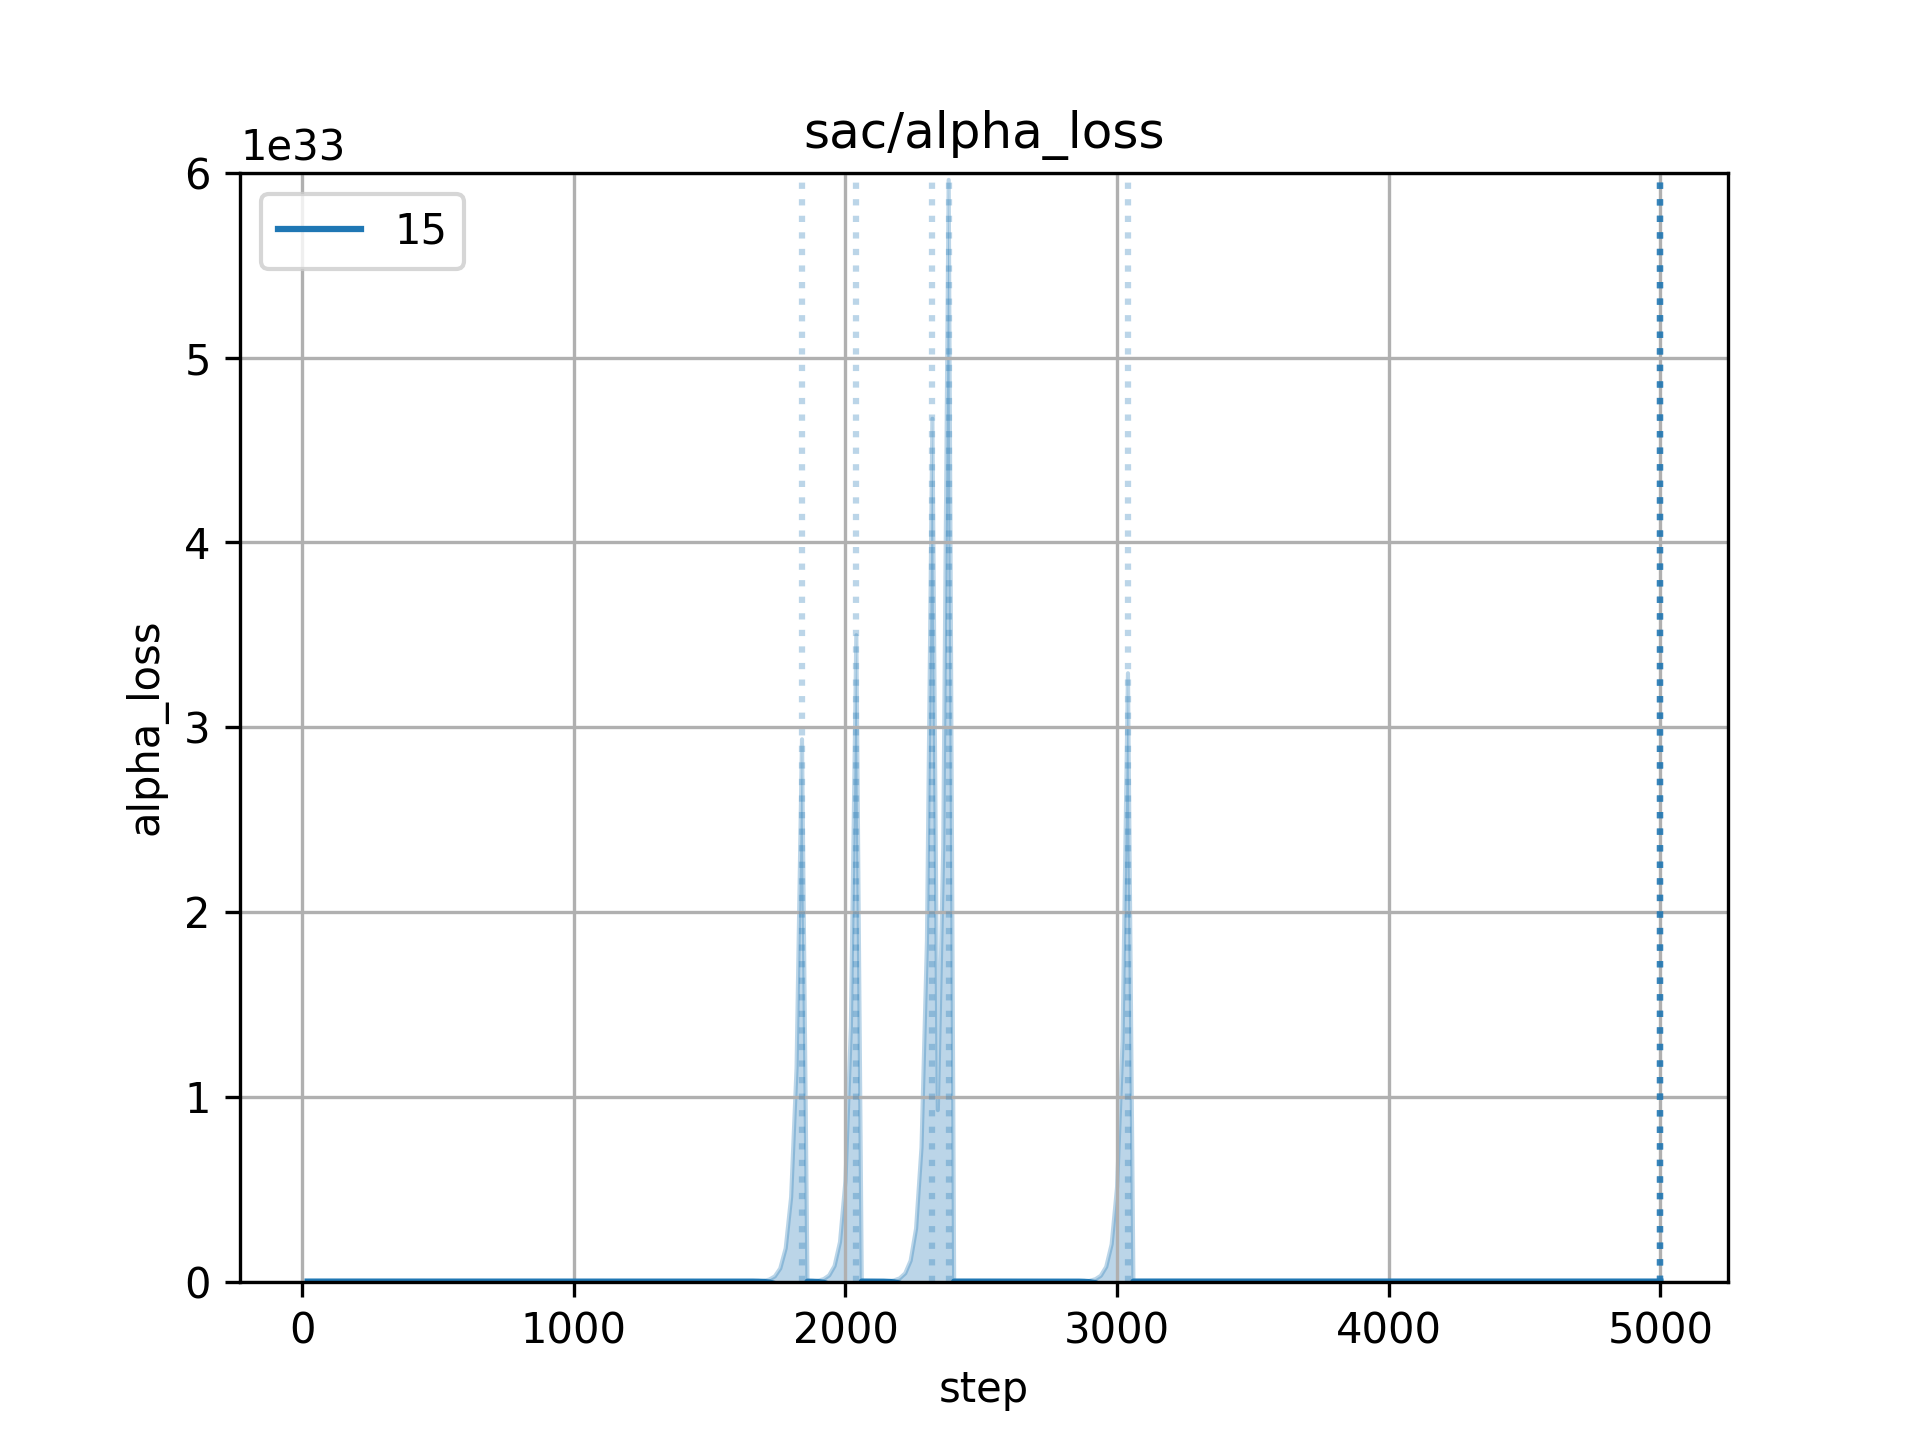
\includegraphics[width=0.23 \linewidth]{figures/appendix/alpha_loss_15.png}
    \end{center}
    \caption[alpha loss with $N = 15$]{Plot to show the correlation between training abortion and spike in alpha loss.}
    \label{fig:alpha_loss_15}
\end{figure}